
\section{Evaluation of Project}
Evaluation of the project consisted of multiple stages ranging from verification of the functional requirements through simple black box testing to evaluation of refined mesh quality using methods provided by Dittmer \cite{DittmerMeshQualityMet}. 

\subsection{Validation against Functional Requirements}
In order to validate the system against many of the functional requirements the system only needs to be run on several basic models with different input configurations. 

% this
output clearly demonstrates the systems ability to evaluate the quality of meshes using a range of metrics and refinement occurring as a result of both the stresses induced by the user and on their categorisation of edges. 


\subsection{Validation against Non Functional}
Validation of non functional requirements was made simple due to the limited number of them, this was partly a consequence of the system not being designed for a specific user base resulting in expectations regarding the systems design to improve usability and guide interaction. It was also not possible to define the general accuracy and performance of the system during the requirement elicitation phase since this could only be determined once the required research and trial on the finished system gave indication to both of these. \\

\noindent
In the case of quality for the systems design and documentation evidence is present to indicate that this adheres to the requirements specified with the project submission containing detailed documentation in the form of a Deoxygen guide and sophisticated use of object oriented and functional software design as seen within the codebase. General applicability of functionality has also been demonstrated through evaluation using a variety of both models and conditions when performing simulations.

\subsection{Unit Testing}
Holistic evaluation provided evidence of the overall systems effectiveness however without verification of individual components it would not have been possible to assess the accuracy of the results generated by the underlying methods. Unit testing was also conducted from within Visual Studio using the NUnit framework and structured as a separate VS project. This provided the guarantee that the system was not able to interact with the tests and that testing was conducted through the class and function interfaces provided by the solution. Tests were grouped into classes with each test class corresponding approximately to one class within the system. Each test class then contains a number of test functions each of which performing the asserts necessary to deem its associated function as correct. This layout provided clear traceability from each item of function to its associated test making assessment of the test coverage much easier.

When designing the tests it was important to not only to 

The design and execution of the tests did manage to reveal a bug within the system . 

Much of the software

 this allowed test names to replicate their partner functions making the 




\subsection{Software Management}
In order to ensure progress was responsibly backed up and features could be easily managed a private Github repository was set up and all progress made to the project pushed every couple of days. This proved invaluable on one occasion where a bug was accidentally introduced and despite efforts could not be removed manually. 
 



\subsection{Software Quality and Maintainability}
The quality of the design and implementation of the system reflects my experience not only as a computer science undergraduate but as a developer with one year industrial experience, although not directly effecting the execution of the program properties such as appropriate variable naming, loose coupling of classes, use of abstractions and descriptive error messages make the software easier to read and debug for any potential future developers. 

Visual Studio also enabled calculation of various software quality metrics for the code base automatically. This made selecting parts of the codebase for refactoring much easier when time was allocated for this. Upon completion of the project the average maintainability index across all modules was 75 with the lowest score for any high level module being 60 and the highest 92. According to the Microsoft Developer Network (MSDN) website code with an index of between 0 and 9 indicates low maintainability, 10 to 19 indicates moderately maintainable and 20 to 100 high maintainabilty \cite{VisualStudioMaintainIndex}.

\subsection{Documentation}
The process of continuously writing descriptive documentation was important to the success of the project and was treated as an integral part to meeting to the goals of the project development methodology which aimed to reduce the systems complexity and improve readability. Through the writing Doc comments corresponding to every function within the codebase it was possible to generate documentation files automatically through use of the tool Doxygen. This allows anyone with the solution to view descriptions of each of its functions either in the codebase or alternatively through the manual produced automatically by Doxygen.



\subsection{Increase in performance through parallel execution}
The following 

The average speed up (Time of serial execution/ Time of parallel execution) was 

The Efficiency of the parallel execution (speedup / number of processors) with an Intel i5 processor with 4 cores the average efficiency  was calculated as

 

\subsection{Evaluation Of System For Model Simulations}

%To demonstrate the systems applicability to a variety of real engineering problems demanded the creation of several models resembling basic equivalents of real structures that are often analysed by FE methods.

several models have been created resembling basic equivalents of that used for real engineering applications.

do this reliably and validate the heuristic component against the results obtained in academic papers two of the three models were based on those previously used by Dolsak (Paper mill and Cylinder structures). In addition to these two a suspension bridge model was developed to demonstrate the systems capacity to work beyond Dolsaks basic validation examples. \\ 

\noindent
These initial models were constructed manually using LISA's graphical user interface using measurements by Dolsak and in the case of the suspension bridge from documents available on the web \cite{DolsakPaper91} \cite{SuspensionBridgeMeasurements}.

\subsubsection{Suspension Bridge structure}

The main model used for testing the methods was a suspension bridge structure. The bridge seemed like a good model to perform initial experimentation on since its structure is 


Constructed manually out of Quad4 LISA elements it has four key constraint points at the base of each supporting column. The bridge itself initially consists of 196 elements and 212 nodes before remeshing, which is considered coarse for such an FE structure. \\


\noindent
When testing the system with the suspension bridge model the first step was to test each method independently of the other in order to evaluate both approaches before attempting to combine the two. Testing each method individually with multiple configurations provided a better understanding of the variation within each allowing more accurate high level reasoning about the results of a hybrid. \\

\noindent
Variation of inputs was particularly important when testing Heuristic method as experimentation revealed a very high amount of variation in the results both in terms of runtime and the methods ability to reveal high stress areas, this can be seen in Figure 9 below. Four main tests were run for the heuristic approach with each test having a different edge specification file of some level of a designated level of quality. With the very good and good edge specifications I made sure to run the model first using stress refinement and then observe areas of high displacement, this allowed specification of edges around areas I knew in advance would benefit from being specified. The idea being a more experienced FE engineer would be able to do this without having to run the stress refinement first. In addition to the two good quality edge specification sets an OK one was also produced where some edges were specified as existing over the highest stress area while others focused mainly on the lower stress areas, and finally a set of poor edges none of which overlapped the high stress area. \\


\begin{figure}[!h]
\centering
\begin{subfigure}{.5\textwidth}
  \centering
  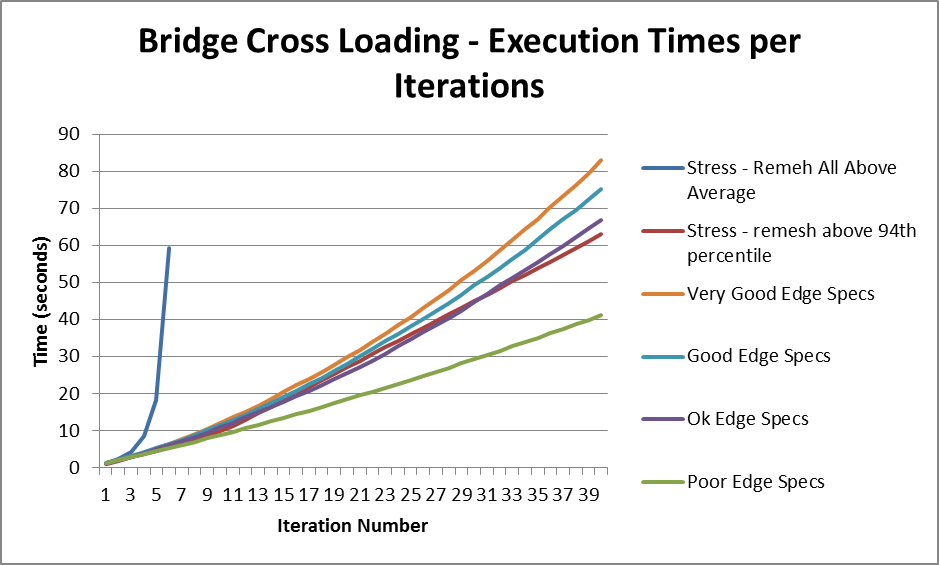
\includegraphics[width=0.9\linewidth]{../Graphics/Graphs/BridgeCrossLoadingExecutionTimesPerIterations.png}
  \caption{Execution time in seconds for each method to reach 40 refinement iterations}
  \label{fig:sub1}
\end{subfigure}%
\begin{subfigure}{.5\textwidth}
  \centering
  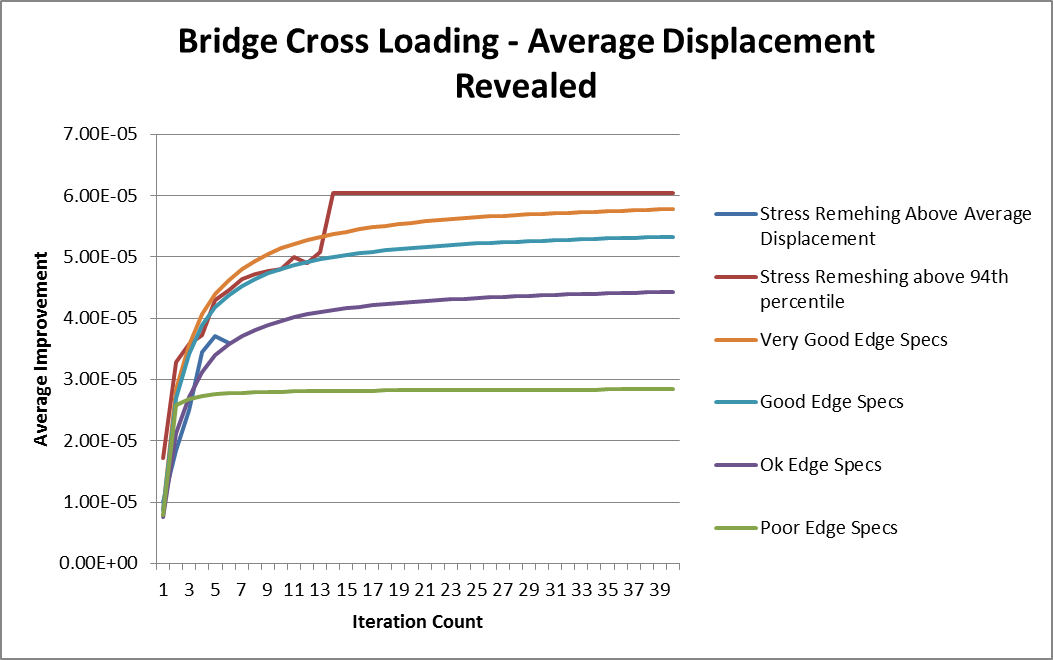
\includegraphics[width=0.9\linewidth]{../Graphics/Graphs/BridgeCrossLoadingAverageDisplacementRevealed.png}
  \caption{Average amount of displacement and thus stress revealed by each approach as number of iterations increases}
  \label{fig:sub2}
\end{subfigure}
\label{fig:test}
  \caption{Execution time increase compared to the amount of information revealed for the different approaches}
 \end{figure}

\noindent
For stress refinement the parameter varied was the threshold used to determine whether elements were considered under high stress and should be further refined. The main consequence of varying this parameter was change in both the node count and the programs runtime. Despite time complexity for subdivision being $O(n^2)$ for all methods using a low threshold results in large values of n and consequently a rapid increase in both runtime and element count. \\

\noindent
In order to perform reasonable comparison between both the stress and heuristic refinement methods it was therefore important to specify the threshold such that approximately equal amounts were performed by each approach per unit of weighting preference per iteration (see combining methods under System Design), thus allowing each method to be evaluated on its merit to select elements appropriately and a hybrid method through its designated weightings. To do this the increase in element count was tracked for the different heuristic methods, as can be seen in Figure 10. The average increase in elements per iteration could then be calculated as 6\% of the total number of elements within the model. This meant stress refinement could be reasonably compared to heuristic refinement if for each use of the refinement it only re meshed those elements considered to be above the 94th percentile in terms of displacement. \\ 


\begin{figure}[!h]
  \centerline{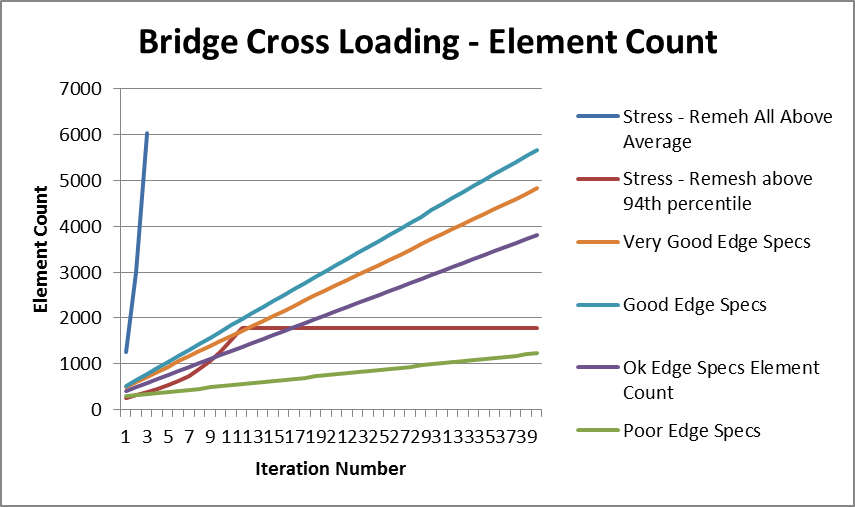
\includegraphics[width=125mm, scale=1]{../Graphics/Graphs/BridgeCrossLoadingElementCount.png}}
  \caption{Execution time in seconds for each method to reach 40 refinement iterations}
  \label{fig:sub1}
\end{figure}

%Having obtained data from multiple runs of the individual methods 
Evaluation of the data Shows that in general refinement based on displacement and stress consistency results in well refined meshes although depending on the threshold this can be highly costly to compute. By contrast heuristics have shown to retain low computational overhead although are volatile when needed to produce meshes of high quality. Where edges are well specified for the heuristics quality can be seen to increase more rapidly than refinement based on displacement data. Heuristic refinement slows down with subsequent iterations which is likely a result of the regions yielding improvement with refinement becoming increasingly small and thus increasing the distance between the edges originally specified and the target meshing location.


Heuristics therefore appear preferable in cases where they can be confirmed as good and where very high accuracy is not as important as reduced computational overhead. By contrast displacement refinement works work well when high accuracy is needed although incurs a higher computational overhead per gain in accuracy early on.

The idea hybrid configuration will therefore exhibit the following two characteristics:

\textbf{Edge Specification assessment:} Establish quickly if the edges specified are any good when meshing, if they aren't stop continued use and switch to displacement refinement.

\textbf{Heuristic Refinement Halting:} If the heuristic refinement does appear to be working well establish at what point it is beginning to become inferior and then switch methods.


Re executing the system with a variety of hybrid weightings 






\subsubsection{Hybrid Evaluation}


\subsubsection{Analysis of and Addition of Metric(s)}
When looking at the initial results of the quality metrics for both the various simulations there were several key observations which greatly informed the remaining evaluation to be conducted. \\ 

The maximum internal angles to elements are one good indication of general quality for the mesh and indeed gradual improvement with additional refinement iterations increasingly subdividing skewed elements into more uniform ones.
Figure 11 below shows greater uniformity towards the optimum of 90 degrees for elements of type Quad4 is achieved for all but the poorest edge specification. Rate of improvement is fast for the first few iterations but then gradually declines 

Looking at the Figure its also clear that as a result of the heuristics being described in terms of edges

\begin{figure}[!h]
  \centerline{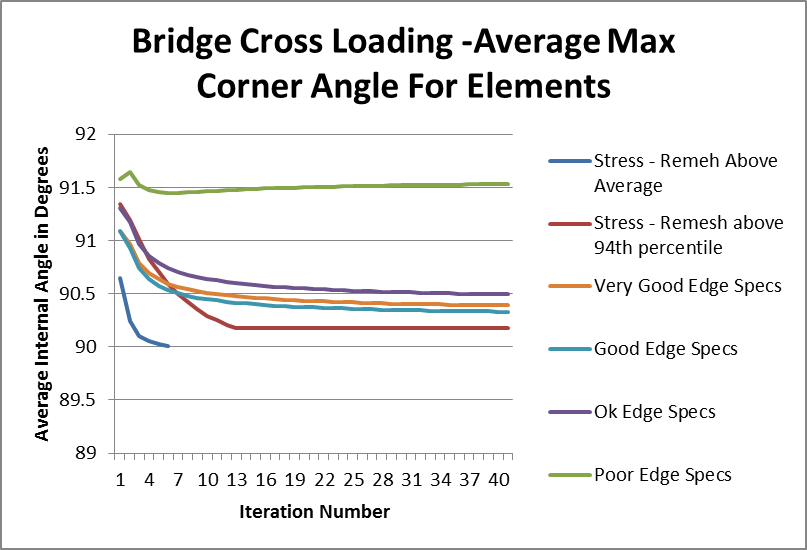
\includegraphics[width=125mm, scale=1]{../Graphics/Graphs/BridgeCrossLoadingAverageMaxCornerAngleForElements.png}}
  \caption{Execution time in seconds for each method to reach 40 refinement iterations}
  \label{fig:sub1}
\end{figure}

Although the Dittmer metrics providing a good indication of general improvement in quality across a mesh or a particular element in the majority of cases they gave little insight into the strengths of a particular element arrangement within a given mesh. Consequently it was possible to conclude using Dittmers metrics that the general quality of the resultant meshes was good with this quality being at lest retained and often improved, but not that the method refining the mesh had made a better selection of elements to mesh. 

\cite{ElemQualAndChecks}. \\


\noindent
It became apparent that for a more conclusive evaluation another metric was also required. To design such a metric I started by reflecting on the fact that each method should provide as much information as possible to an engineer while retaining the lowest computational overhead possible, essentially what much additional information is revealed through each additional iteration of a given approach. It can also assume in this case that the concentration of displacement and therefore stress is what we are interested in finding. I concluded that the best means of evaluating each method was was to cross reference the resultant stress data for each iteration against the newly refined regions generated by each approach, the overall stress revealed within the output as a result of that part of the mesh being refined could then be summed and divided by the number of nodes created in order to reveal it through evaluation. This new metric became the average displacement revealed metric as can be seen in Figure 9b.




%\begin{figure}{\textwidth}
%  \centering
%  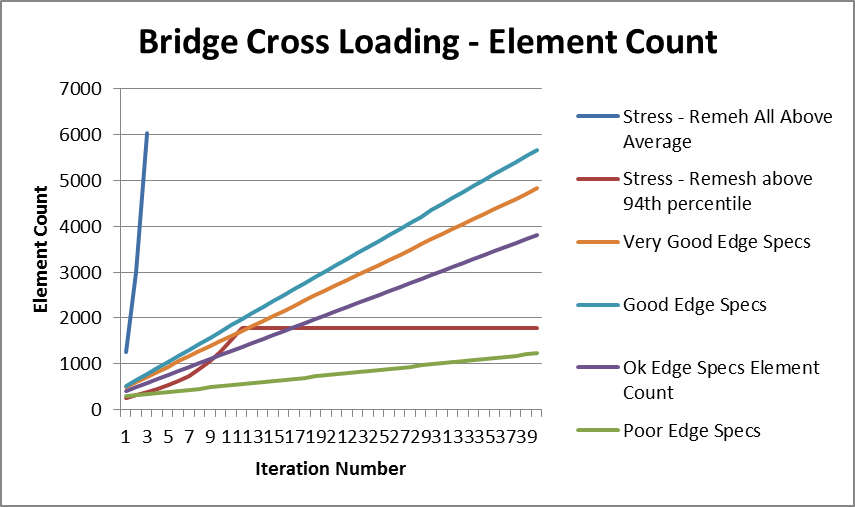
\includegraphics[width=0.9\linewidth]{../Graphics/Graphs/BridgeCrossLoadingElementCount.png}
%  \caption{Execution time in seconds for each method to reach 40 refinement iterations}
%  \label{fig:sub1}
%\end{figure}
%see appendix x figure for example

\noindent
%Currently the default setting for the evaluation function is to refine any elements with a stress greater than the 94th percentile for the model. The threshold setting is relatively arbitrary although choosing to mesh elements rated above the 94th percentile allowed the stress refinement method to be fairly compared against the heuristic methods since these typically only selected about 6\% of elements for refinement although this can clearly vary depending on the model and edges used.


% of input configurations was particularly important when analysing the heuristic method since  by what edges were provided to it by the operator.


%When testing the stress refinement method the main approach altered






In order to evaluate general consistency in these results the experiments were rerun for 


Results for which can be seen in 


\newpage
\subsection{Evaluation of Subsystems based on model evaluation}
Running the system for the above models gave clear indications as to the overall effectiveness of both methods

Having run the system on the range of models described above it was possible to begin assessing it's ability to mesh and the use of Dittmers metrics for assessing 
the quality of each mesh.

\subsubsection{Analysis of Methods Using Metrics}
When evaluating Dittmers metrics for distinguishing between meshes of different qualities there were several key observations that resulted in re assessment of how to evaluate the mesh qualities in general.



\iffalse
%graphs of Dittmer metrics showing little variation in the results
\begin{figure}[!h]
\centering
\begin{subfigure}{.5\textwidth}
  \centering
  \includegraphics[width=0.9\linewidth]{g}
  \caption{Cylinder model used by Dolsak with edges labeled, each labelling corresponds to a rule generated by the Golem algorithm \cite{DolsakPaper91}}
  \label{fig:sub1}
\end{subfigure}%
\begin{subfigure}{.5\textwidth}
  \centering
  \includegraphics[width=0.9\linewidth]{}
  \caption{Diagram representing the general structure of the system with interactions between non internal entities such as files and LIA shown using dashed lines}
  \label{fig:sub2}
\end{subfigure}
\label{fig:test}
\end{figure}
\fi



\noindent
Having coded this into the MeshQualityAssessment class the results for this metric could be plotted to evaluate each approach over a number of iterations for the different simulations. I also varied the selection of edges provided to heuristic refinement method which highlighted just how dependent the heuristic approach was on the quality of user expertise.

\begin{figure}[!h]
\centering
\begin{subfigure}{.5\textwidth}
  \centering
  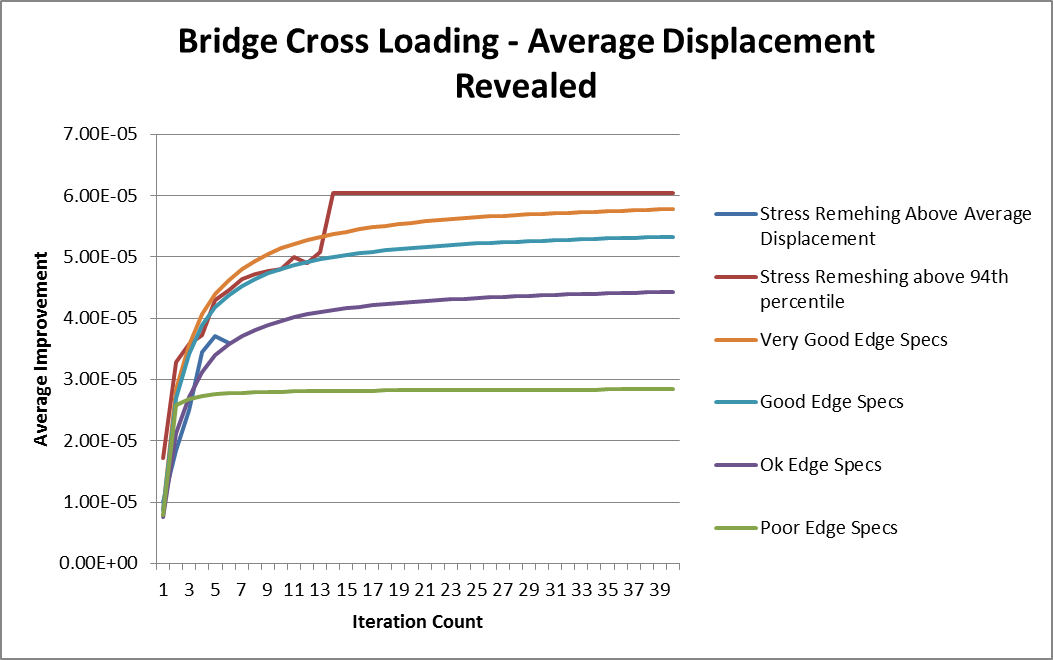
\includegraphics[width=0.9\linewidth]{../Graphics/Graphs/BridgeCrossLoadingAverageDisplacementRevealed.png}
  \caption{Bridge Cross Loading -Average Displacement Revealed Through Creation of Node per Iteration the plateau experienced by Stress Remeshing above 94th percentile is a consequence of all subsequent meshing being focused on an area already very highly meshed, in other words}
  \label{fig:sub1}
\end{subfigure}%
\label{fig:test}
\end{figure}

%Subsequent research suggested


%Demonstrating potential for both heuristic and hybrid refinement for small models suggests that there is still a large amount of work to be done in this area. Although extensive work has been done by engineers and mathematicians to improve the numerical methods associated with the method for many years the improvements obtained  


\subsubsection{Evaluation of Stress Refinement Effectiveness}
Comparisons across multiple models suggests that for general purpose scenarios where results of the simulation are highly unpredictable and the geometry irregular stress based refinement will continue to provide engineers with reliable results within a predictable although potentially costly amount of time. This scenario likely encapsulates the majority of use cases for FE analysis in the real world and therefore is likely to remain the prominent approach by practitioners.

It is clear however that the decline in performance is dependent upon the threshold used to detemine meshing

\subsubsection{Evaluation of Heuristic Refinement Effectiveness}
The most crucial observation which can be made through analysis of the simulation data is that heuristic equation based on model edges has resulting mesh quality has high variability. Despite this it is also clear that despite high variation in results for different edge specifications the general rate of growth or decline for the resultant metric values remains consistent.


\subsubsection{Evaluation Issues}
A significant issue faced in attempting to demonstrate the effectiveness of the system was to provide an indication of how well the system worked without taking into account the ability of the user who may be providing the edge rules for a particular model. Not taking this into account would result in an inaccurate representation of its ability.

\subsection{Strengths and Weaknesses}

The resulting system successfully satisfied both the functional and non functional requirements in addition to providing insights into the possibilities of a hybrid technique for effective finite element meshing, something that was optimistic at the start of the project but highly desirable. The project was well managed with deliverables consistent met as per the initial time plan quality maintained through application of good software engineering practice. \\
 


\noindent
One of the great strengths of the system would be its modular architecture which has allowed for a great amount of potential extendibility in the future. Although little focus has so far been given to the systems usability it can ideally be developed and distributed as tool for experimentation with hybrid meshing with limited additional effort. \\

\noindent
Another strength of the system is its ability to accept any heuristic definition in terms of edges within a mesh structure. Theoretically this means the final system is also capable of using the same types of edge specifications for any type of FE analysis such as fluid flow or heat transfer given a corresponding rule set by which to mesh with. \\


\noindent
A downside of the current design is manual specification of the edges by the user directly into the JSON input file which is both time consuming and prone to error despite the relatively small size of the models analysed in this dissertation. Comparing the size of these with those those used in industry it is clear that this process is simply not practical for engineers conducting FE analysis. To change this better tools are required that will allow engineers to automatically generate edge specifications quickly, most likely through some GUI or a bespoke high level language capable of combining knowledge about the mesh structure and different types of edges to generate specific rules. Again this is beyond the scope of the project and would likely be a dissertation in its own right. \\


\noindent
Although the system had a strong subsystem and class level architecture many of its greater weaknesses could be attributed to prioritisation of its rapid prototyping over efficient implementation of the various algorithms and methods described in this dissertation. Much of this a consequence of overusing the functional programming capabilities within the C\# LINQ library. Widespread adoption of functional programming practices was stated as a desirable aspect of the final system implementation within the original non functional requirements. This has largely been adhered to with  higher order and lambda functions widespread throughout the codebase. In the later stages of the project it became apparent however that in many cases reliance on these features resulted in reduced readability and performance for many of underlying algorithms described in this dissertation. \\

One such 

One such example where functional programming was 


In many cases over reliance on map resulted in


As a consequence of trying to embrace the functional programming style as part of a practical software development project 




Additionally the system demonstrated also proved capable of providing interesting insights into the possibilities of performing hybrid and even demonstrated that 

% Overall the project met all its initial requirements laid out in both the objectives and its requirements.
% Sould have done test driven development to ease testing at the end


\subsection{Evaluation summary}



\subsection{Successes and Limitations of project}
Having reflected on the the results of the methods implemented within the system through the execution of
